\documentclass[10pt]{article}
\usepackage[margin=0.76in]{geometry}
\usepackage{amsmath,amssymb,booktabs,graphicx,microtype,xcolor,float}
\usepackage[T1]{fontenc}
\usepackage{lmodern}
\usepackage[colorlinks=true,allcolors=blue!55!black]{hyperref}
\setlength{\parindent}{0pt}
\setlength{\parskip}{5pt}
\newcommand{\roadmapstep}[2]{%
  \fcolorbox{blue!55!black}{blue!5}{%
    \parbox[c][0.72in][c]{1.22in}{\centering\small\textbf{#1}\\[2pt]\footnotesize #2}}}
\title{The Work of Reducing Dependence}
\author{J. R. Landers}
\date{September 2026}
\begin{document}
\maketitle

\begin{abstract}
Can we predict the work needed to make two physical systems less dependent, then check the prediction against an experiment? We begin with the pointwise dependence ratio $R=p_{12}/(p_1p_2)$, where $p_{12}$ is the joint probability density and $p_1,p_2$ are its marginals. We use its average log, mutual information $I$, to measure overall dependence. A solvable equilibrium model predicts exactly that a slow reduction of $I$ by $\Delta I$ costs $k_BT\Delta I$ of work. We then examine two cavity-coupled membranes as a possible test of the same dependence-and-work question. Their published coupling and heat-flux measurements constrain the model, but the real device has two baths and an optical spring that changes each membrane's frequency, so its work cannot be inferred from $\Delta I$ alone. In that model, lowering coupling reduces position dependence while increasing dependence carried by the heat current. It still requires positive control work. Existing figures check the heat-flux scale but do not report the joint motion and control work needed to test these predictions. We state the required measurements explicitly.
\end{abstract}

\begin{center}
\small\textbf{From a mathematical dependence change to an experimental test}\\[6pt]
\roadmapstep{Define the dependence change}{$R$ and $\Delta I$}
\hspace{2pt}$\rightarrow$\hspace{2pt}
\roadmapstep{Calculate work}{$W_{\rm rev}=k_BT\Delta I$}
\hspace{2pt}$\rightarrow$\hspace{2pt}
\roadmapstep{Model membranes}{Two baths and optical spring}
\hspace{2pt}$\rightarrow$\hspace{2pt}
\roadmapstep{Propose a test}{Joint motion and control work}
\end{center}

\section{Dependence and work}
Let $x$ and $y$ denote simultaneous position measurements of two oscillators. Write $p(x,y)$ for their joint probability density and $p_1(x)$ and $p_2(y)$ for its marginals. Their pointwise dependence ratio $R$ and mutual information $I$ are
\begin{equation}
 R(x,y)=\frac{p(x,y)}{p_1(x)p_2(y)},\qquad
 I=\langle\log R\rangle
 =\iint p(x,y)\log R(x,y)\,dx\,dy . \label{eq:ratio}
\end{equation}
The brackets $\langle\cdot\rangle$ denote an average under the joint density $p(x,y)$. If the positions are independent, $R=1$ almost everywhere and $I=0$. For dependent positions, $R$ may be above one in some regions and below one in others. The average in Eq.~\eqref{eq:ratio} is their Kullback--Leibler divergence from the product distribution, in nats. We use $I$ to compare overall dependence and $R$ to locate changes within the state space.

For a chosen pair of observables, define the before-to-after change as $\Delta I=I_{\rm before}-I_{\rm after}$. A positive $\Delta I$ means that the protocol reduces their dependence. We ask what signed work $W_{\rm on}$ is done on the system to produce that change, taking positive work to mean energy supplied to the system. The ratio $R$ describes each state, but work depends on the controlled Hamiltonian, baths, and path between states. We first answer the question exactly in a one-bath model, then apply the same dependence measure to a membrane system that needs a different work calculation.

\section{Equilibrium prediction}
To calculate a work cost for the $\Delta I$ defined above, we start with two classical oscillators in one bath at temperature $T$. Each has uncoupled stiffness $k>0$, and the tunable cross-stiffness is $g$. Their controlled potential is
\begin{equation}
 V_\times(x,y)=\frac{k}{2}(x^2+y^2)+gxy,\qquad q=g/k,\quad |q|<1 . \label{eq:cross}
\end{equation}
The dimensionless $q$ measures the cross-coupling relative to each spring; $|q|<1$ keeps the potential stable.
With $k_B$ denoting Boltzmann's constant, the Gibbs distribution has covariance $k_BT\left(\begin{smallmatrix}k&g\\g&k\end{smallmatrix}\right)^{-1}$. Its position correlation coefficient is $\rho=-q$. Gaussian integration then gives
\begin{equation}
 \rho=-q,\qquad I(q)=-\frac12\log(1-q^2),\qquad
 W_{\rm rev}=k_BT[I(q_{\rm before})-I(q_{\rm after})].
 \label{eq:benchmark}
\end{equation}
Here $W_{\rm rev}$ is the reversible work done on the oscillators. For a quasistatic isothermal change, it equals the change in Helmholtz free energy $F$. In this model $F(q)-F(0)=(k_BT/2)\log(1-q^2)=-k_BT I(q)$ (Appendix~\ref{app:equilibrium}), which yields Eq.~\eqref{eq:benchmark}. As $|q|$ decreases, $I$ falls and $F$ rises. This equality follows from the specified potential and bath; it is not a general conversion from information to work.

Yang \emph{et al.} report two membrane modes with uncoupled angular frequency $\omega_0$, where $\omega_0/2\pi=400$ kHz, and tunable cavity-mediated coupling rate $\Lambda$.\cite{yang2020} Mapping their measured normal-mode splitting onto the cross-coupling model gives $|q|\simeq2|\Lambda|/\omega_0$; using $|q|\simeq|\Lambda|/\omega_0$ would miss a factor of two. With the correct mapping, a change from $|\Lambda|/2\pi=85$ to $58$ Hz in the \emph{equal-temperature cross-coupling model} would give $\Delta I=4.83\times10^{-8}$ nats and $W_{\rm rev}=2.00\times10^{-28}$ J at 300 K. These numbers establish a benchmark for the same before-and-after coupling values; they are not the work cost of the membrane apparatus.

\section{Modeling the membranes}
We now ask what happens to dependence and work for that same 85 to 58 Hz change in the membranes. Two features prevent us from using Eq.~\eqref{eq:benchmark} as their work prediction. One membrane is driven by added white noise while the other contacts a room-temperature bath, producing a nonequilibrium steady state with heat flow.\cite{yang2020} The cavity also shifts each mode's frequency along with their coupling. Let $m$ be the effective mode mass, $x_i$ its position, and $p_i=m\dot x_i$ its momentum; here $p_i$ is distinct from the probability densities in Eq.~\eqref{eq:ratio}. An effective classical Hamiltonian consistent with the reported mode matrix to first order in $|\Lambda|/\omega_0$ is
\begin{equation}
 H_{\rm opt}=\frac{p_1^2+p_2^2}{2m}
 +\frac{m\omega_0^2}{2}(x_1^2+x_2^2)
 +m\omega_0\Lambda(x_1+x_2)^2 . \label{eq:opt}
\end{equation}
Writing the dimensionless optical-spring strength as $h=2\Lambda/\omega_0$, its stiffness matrix is $m\omega_0^2\left(\begin{smallmatrix}1+h&h\\h&1+h\end{smallmatrix}\right)$. The normal frequencies are $\omega_0$ and $\omega_0\sqrt{1+2h}$, reproducing the observed splitting to first order. At equal temperature the Helmholtz free energy $F_{\rm opt}$ of this optical-spring model changes by
\begin{equation}
 F_{\rm opt}(h)-F_{\rm opt}(0)=\frac{k_BT}{2}\log(1+2h). \label{eq:optfree}
\end{equation}
For the slow 85 to 58 Hz change, Eq.~\eqref{eq:optfree} gives $5.60\times10^{-25}$ J at 300 K, about 2800 times the cross-only benchmark. Even at equal temperature, the same change in coupling has a different work cost because the local spring shifts in Eq.~\eqref{eq:opt} contribute at first order in $h$, while position dependence changes only at second order (Appendix~\ref{app:equilibrium}).

With two baths, we calculate the joint fluctuations generated by Eq.~\eqref{eq:opt}. At each coupling, $R_{\rm pos}$ is Eq.~\eqref{eq:ratio} with $x=x_1$ and $y=x_2$. The same joint-to-product density ratio defines $R_{\rm ph}$ for the full oscillator states $\boldsymbol{\xi}_i=(x_i,\dot x_i)$. Their mutual informations are $I_{\rm pos}=\langle\log R_{\rm pos}\rangle$ and $I_{\rm ph}=\langle\log R_{\rm ph}\rangle$, each averaged over its corresponding joint distribution. The latter includes the position--velocity correlation associated with heat transport. For resonant modes, weak optical-spring shifts, and independent Gaussian bath forces, a rotating-wave calculation links it to the mean heat current $J$. Let $T_i^{\rm eff}$ be the steady-state temperature inferred from mode $i$'s variance. Then
\begin{equation}
 I_{\rm ph}=-\log(1-r_J^2),\qquad
 r_J=\frac{|J|}{2|\Lambda|k_B\sqrt{T_1^{\rm eff}T_2^{\rm eff}}}.
 \label{eq:current}
\end{equation}
The dimensionless $r_J$ is the magnitude of the normalized cross-correlation between mode amplitudes. Equation~\eqref{eq:current} can therefore estimate $I_{\rm ph}$ from $J$, $\Lambda$, and the two effective temperatures. Measuring the joint covariance would allow $R_{\rm ph}$ and $I_{\rm ph}$ to be reconstructed more directly, without relying on the rotating-wave approximation (Appendix~\ref{app:steady}).

\begin{samepage}
Let $T_H$ and $T_L$ be the hot- and cold-bath temperatures, with oscillator 1 coupled to the hot bath and oscillator 2 to the cold bath. For scale, take $T_H/T_L=430$, approximately the hot-bath level in the published temperature plot. We solve the full linear Langevin covariance equation, including terms omitted from Eq.~\eqref{eq:current}. At the two reported coupling values, the model predicts
\begin{center}
\begin{tabular}{lrr}
\toprule
Predicted quantity&85 Hz&58 Hz\\
\midrule
$I_{\rm pos}$ (nats)&$9.05\times10^{-8}$&$4.22\times10^{-8}$\\
$I_{\rm ph}$ (nats)&$0.00123$&$0.00264$\\
Mean heat current (W)&$4.45\times10^{-17}$&$4.44\times10^{-17}$\\
\bottomrule
\end{tabular}
\end{center}
\end{samepage}
Using the before-minus-after convention of Section 1, $\Delta I_{\rm pos}=4.83\times10^{-8}$ nats, whereas $\Delta I_{\rm ph}=-1.41\times10^{-3}$ nats. The positions become less dependent, but the full oscillator states become more dependent. A weaker coupling sustains a larger temperature difference, and the position--velocity correlation associated with heat transport becomes more prominent relative to each oscillator's fluctuations. Thus a claim of reduced dependence must specify the observed variables.

Figure~\ref{fig:ratio} shows pointwise ratios for two pairs of observables. The lower row is a position--velocity marginal that illustrates one contribution to $I_{\rm ph}$; it is not the full-state ratio $R_{\rm ph}$. Within each row the same color scale is used at both coupling settings. The position ratio moves closer to one as coupling falls; the position--velocity ratio moves further from one. Neither ratio changes in the same direction at every point. Mutual information summarizes the average log ratio, not a pointwise ordering.
\begin{figure}[H]
\centering
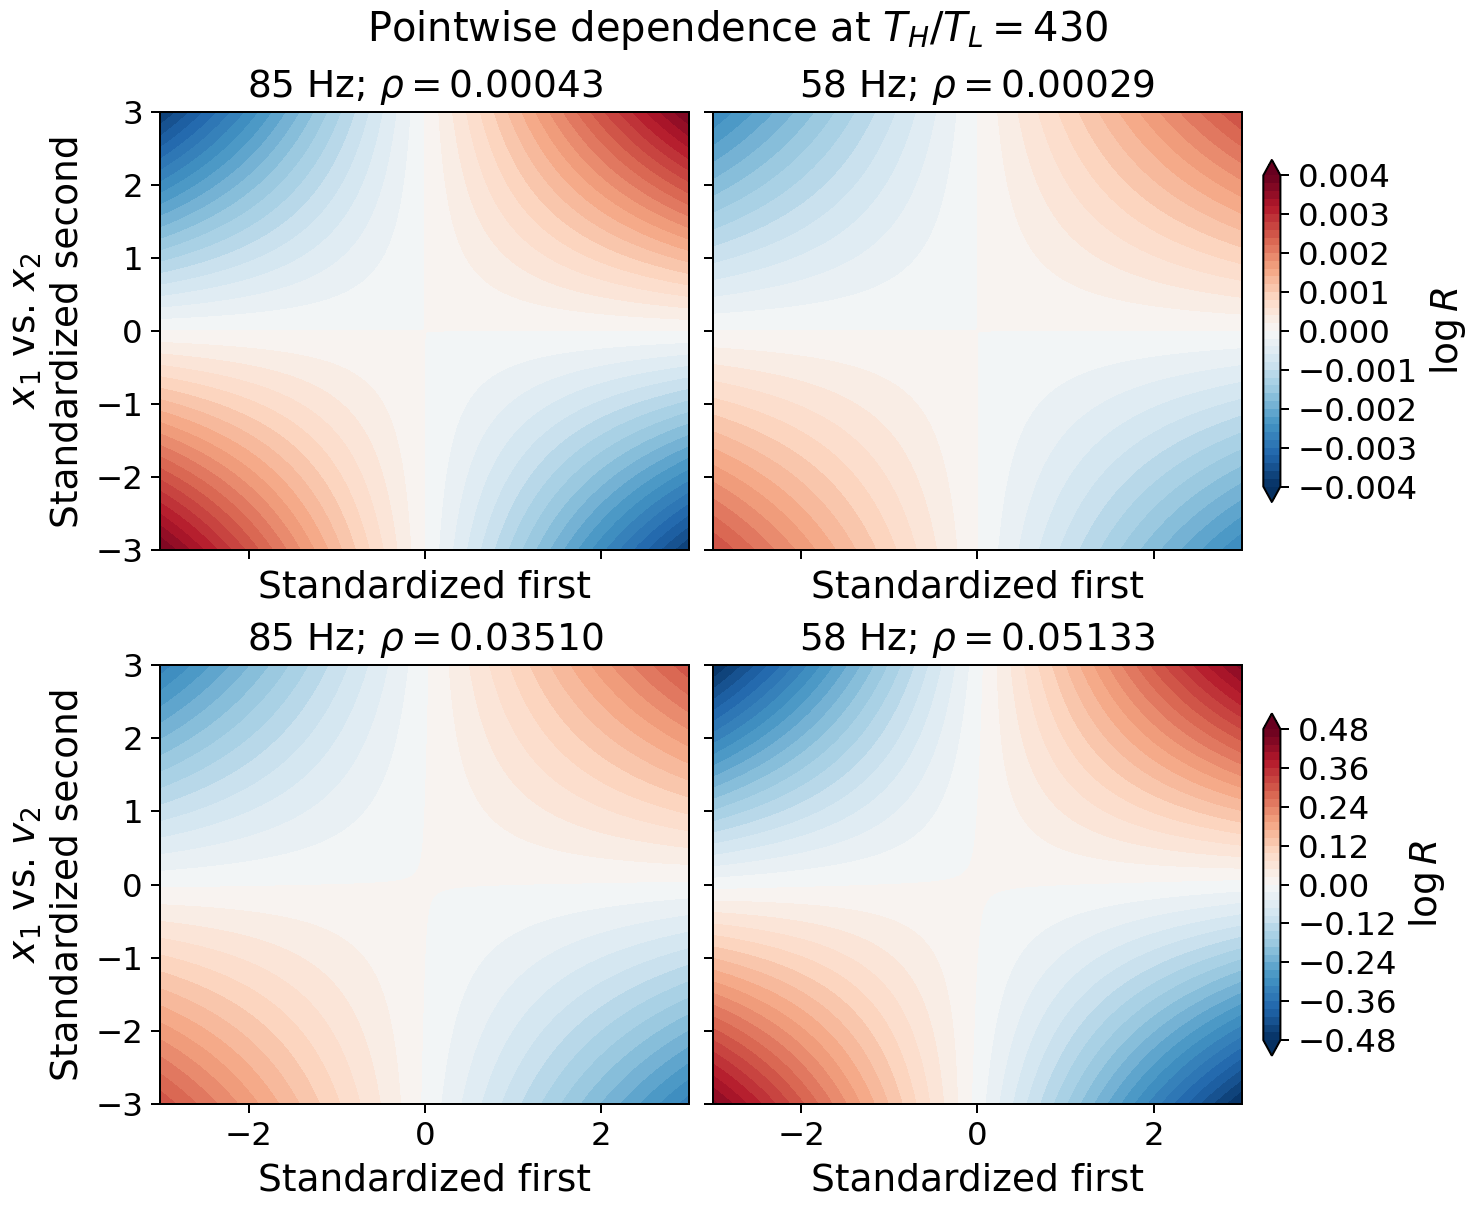
\includegraphics[width=0.72\linewidth]{optical_spring_results/pointwise_ratio_landscapes.png}
\caption{Predicted pointwise log ratios for standardized $(x_1,x_2)$ and $(x_1,\dot x_2)$ readings. These are two-variable marginals of the model, not reported experimental histograms.}
\label{fig:ratio}
\end{figure}

\newpage
Having identified both dependence changes, we calculate the work for the same coupling protocol. The equilibrium identity in Eq.~\eqref{eq:benchmark} cannot supply that work; differentiating the controlled Hamiltonian in Eq.~\eqref{eq:opt} with respect to $\Lambda$ instead gives
\begin{equation}
 W_{\rm on}=m\omega_0\int \dot\Lambda(t)
 \left\langle[x_1(t)+x_2(t)]^2\right\rangle dt . \label{eq:work}
\end{equation}
Here $\dot\Lambda=d\Lambda/dt$, and the brackets average over the evolving oscillator state. That average must be known \emph{throughout} the protocol.
We evolve the Gaussian covariance during linear 85 to 58 Hz ramps lasting $0.1$ ms to $1$ s, each initialized in the 85 Hz steady state (Appendix~\ref{app:dynamics}). All ramps require positive work on the \emph{effective mechanical Hamiltonian}. For $T_H/T_L=430$, the 1 s result is $1.60\times10^{-22}$ J at $T_L=300$ K. It exceeds the cross-only benchmark because local spring terms contribute at first order in $\Lambda$ and the hot bath increases fluctuations. It excludes laser power and heat spent maintaining the steady state; the experiment did not report this ramp. Figure~\ref{fig:work} separates total work from the smaller effect of ramp duration.
\begin{figure}[H]
\centering
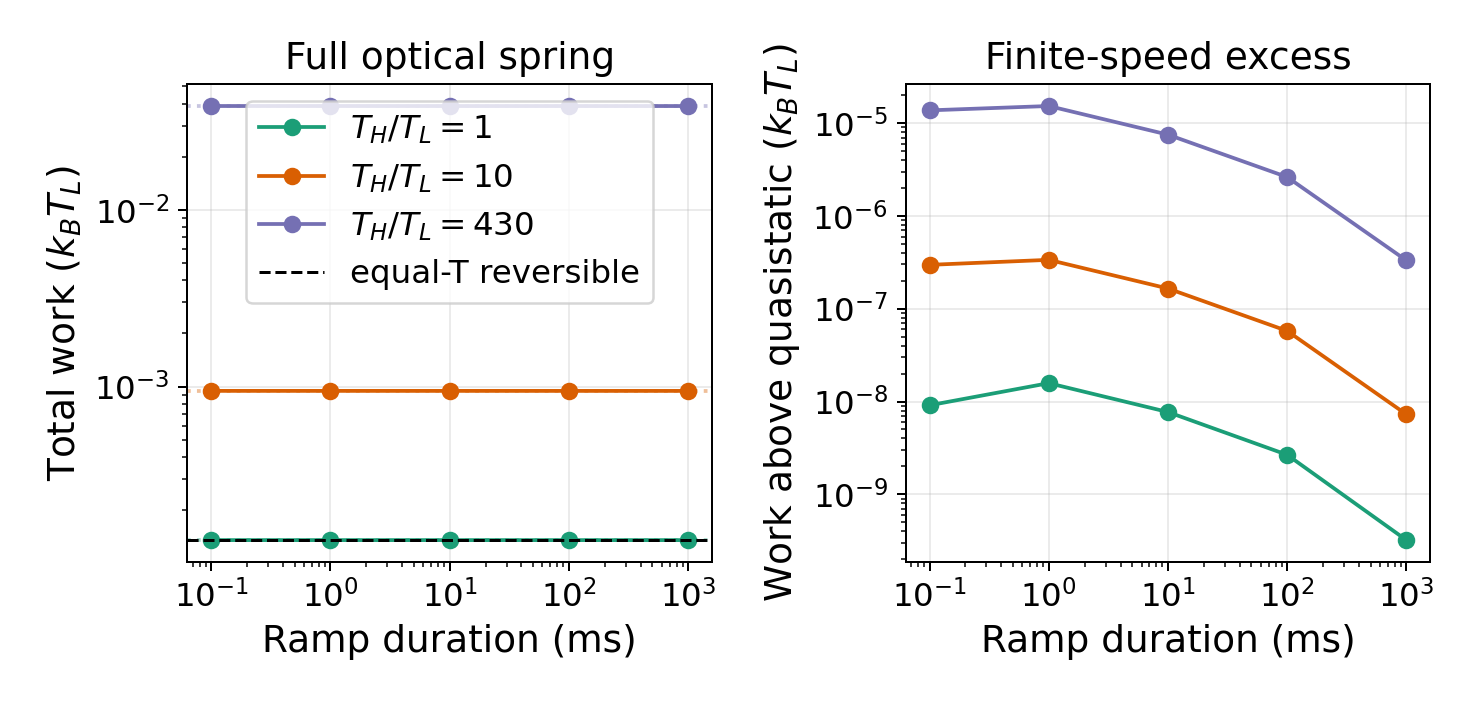
\includegraphics[width=0.68\linewidth]{optical_spring_results/work_vs_duration.png}
\caption{Predicted work for the 85 to 58 Hz change. Total work (left) is dominated by the optical spring's local frequency shift. The right panel subtracts the integral of the steady-state generalized force along the same path, exposing finite-speed excess. This reference is a free-energy difference only when the baths have equal temperatures. None of these curves are measured apparatus power.}
\label{fig:work}
\end{figure}

\section{Experimental test and existing evidence}
Existing measurements provide partial checks of the membrane model. The published normal-mode splitting and heat-flux oscillation frequency support the coupling scale $2|\Lambda|$.\cite{yang2020} The measured mean heat flux approaches roughly $4\times10^{-17}$ W; using the approximate bath ratio above, the model predicts a saturation scale of $4.46\times10^{-17}$ W. This is an order-of-magnitude check, not a fit to source data. The published temperature curves also approach one another as coupling grows, as the model predicts qualitatively. The reported high-power temperatures appear below our simple model's $\simeq287\,T_L$ prediction, so that comparison remains unresolved.

Testing the predicted dependence and work changes requires synchronized joint motion data and a calibrated 85 to 58 Hz work protocol, neither of which is reported in the public article. Its data and code are available from the authors on request.\cite{yang2020} A direct comparison would reconstruct $R_{\rm pos}$ and $R_{\rm ph}$ from both membrane quadratures at several couplings, calculate their average logs, and record the control trajectory and energy flows during the coupling change. The measured covariance, heat current, and work could then be compared with Eqs.~\eqref{eq:gaussianratio}, \eqref{eq:current}, and \eqref{eq:work} at the same settings. Such a measurement would test the membrane-specific predictions; it would not by itself establish the equilibrium identity in Eq.~\eqref{eq:benchmark}.

\section{Conclusion}
The theory gives an exact work--information prediction for a clean equilibrium benchmark. Asking the same before-and-after question for the membranes reveals a sharper test: identify \emph{which} dependence is being reduced, include the local optical spring in the work calculation, and measure both the joint state and control energy. Published results check parts of the transport model, but they do not yet test the predicted dependence and work changes. This analysis is classical; entanglement would require a separate quantum treatment of the same question.

\paragraph{Reproducibility.} Run \texttt{optical\_spring\_sweep.py} for the finite-time CSV and figures.\par
Run \texttt{extensions\_calculations.py} for the equilibrium and steady-state values. The equations and covariance method are detailed in the earlier working notes and the experiment's Supplementary Information.\cite{yangsupp}

\appendix
\section{Equilibrium calculations}\label{app:equilibrium}
For Eq.~\eqref{eq:cross}, the stiffness and position covariance matrices are
\begin{equation}
 K_\times=k\begin{pmatrix}1&q\\q&1\end{pmatrix},\qquad
 C_\times=k_BT K_\times^{-1}
 =\frac{k_BT}{k(1-q^2)}
 \begin{pmatrix}1&-q\\-q&1\end{pmatrix}.
\end{equation}
The kinetic partition function is independent of $q$, whereas the position partition function is proportional to $(\det K_\times)^{-1/2}$. Hence $F_\times(q)-F_\times(0)=(k_BT/2)\log(1-q^2)=-k_BT I(q)$, proving Eq.~\eqref{eq:benchmark}.

For any zero-mean Gaussian pair standardized to unit variance, with correlation coefficient $\rho$, the pointwise ratio is
\begin{equation}
 \log R_\rho(a,b)=-\frac12\log(1-\rho^2)
 +\frac{\rho ab-\frac12\rho^2(a^2+b^2)}{1-\rho^2}.
 \label{eq:pairratio}
\end{equation}
This is the function shown in Fig.~\ref{fig:ratio}; averaging it over the joint Gaussian gives $I=-\frac12\log(1-\rho^2)$. Its sign can change across $(a,b)$ even when $I>0$.

For Eq.~\eqref{eq:opt}, let $h=2\Lambda/\omega_0$. Then $K_{\rm opt}=m\omega_0^2\left(\begin{smallmatrix}1+h&h\\h&1+h\end{smallmatrix}\right)$, with determinant $(m\omega_0^2)^2(1+2h)$. Its equilibrium position correlation is $\rho_{\rm pos}=-h/(1+h)$, so
\begin{equation}
 F_{\rm opt}(h)-F_{\rm opt}(0)=\frac{k_BT}{2}\log(1+2h),\quad
 I_{\rm pos}(h)=-\frac12\log\left[1-\left(\frac{h}{1+h}\right)^2\right].
\end{equation}
For small $|h|$, the work change is first order in the change of $h$, while $I_{\rm pos}=h^2/2+O(h^3)$. This explains why the optical-spring work cannot be inferred from Eq.~\eqref{eq:benchmark}.

\section{Steady-state covariance}\label{app:steady}
The experiment's resonant effective-mode equation has a coupling $\Lambda$ both on and off its diagonal.\cite{yang2020} In the rotating-wave approximation, let $b_i$ be the complex amplitude of mode $i$ and $\gamma_i$ its damping rate. With $T_1=T_H$, $T_2=T_L$, and $\hbar$ the reduced Planck constant, define the bath occupations $n_i=k_BT_i/(\hbar\omega_0)$, the steady occupations $N_{ii}=\langle|b_i|^2\rangle$, and $s=\operatorname{Im}\langle b_1b_2^*\rangle$. The steady solution is
\begin{align}
 s&=\frac{2\Lambda\gamma_1\gamma_2(n_1-n_2)}
 {(\gamma_1+\gamma_2)(\gamma_1\gamma_2+4\Lambda^2)},\nonumber\\
 N_{11}&=n_1-\frac{2\Lambda s}{\gamma_1},\qquad
 N_{22}=n_2+\frac{2\Lambda s}{\gamma_2},\qquad
 J=2\hbar\omega_0\Lambda s .
 \label{eq:rwa}
\end{align}
The real cross-correlation vanishes at exact resonance. The effective mode temperatures satisfy $k_BT_i^{\rm eff}=\hbar\omega_0N_{ii}$, so writing $r_J=|s|/\sqrt{N_{11}N_{22}}$ gives Eq.~\eqref{eq:current}. The phase-space mutual information is $-\log(1-r_J^2)$ because the two quadrature pairs have the same correlation magnitude.

For the numerical calculations we retain the full position and velocity dynamics. In dimensionless coordinates $z=(u_1,v_1,u_2,v_2)$, with $u_i=\omega_0x_i/\sqrt{k_BT_L/m}$ and $v_i=\dot x_i/\sqrt{k_BT_L/m}$, the covariance $C=\langle zz^{\mathsf T}\rangle$ satisfies a linear equation with drift matrix $A$ and diffusion matrix $D$:
\begin{equation}
 \dot C=A(h)C+CA(h)^{\mathsf T}+D,\quad
 A(h)=\begin{pmatrix}
 0&\omega_0&0&0\\
 -\omega_0(1+h)&-\gamma_1&-\omega_0h&0\\
 0&0&0&\omega_0\\
 -\omega_0h&0&-\omega_0(1+h)&-\gamma_2
 \end{pmatrix},\quad
 D=\operatorname{diag}(0,2\gamma_1T_H/T_L,0,2\gamma_2).
 \label{eq:covode}
\end{equation}
The steady state solves $AC+CA^{\mathsf T}+D=0$. Partition $C$ into the two oscillator blocks $C_1,C_2$. Gaussian integration then gives
\begin{equation}
 I_{\rm ph}=\frac12\log\frac{\det C_1\det C_2}{\det C},\quad
 \log R_{\rm ph}(z)=I_{\rm ph}
 -\frac12z^{\mathsf T}
 \left[C^{-1}-\operatorname{diag}(C_1^{-1},C_2^{-1})\right]z .
 \label{eq:gaussianratio}
\end{equation}
The same formulas applied to the $2\times2$ position submatrix give $I_{\rm pos}$ and $R_{\rm pos}$. These definitions show why two distributions with different observed variables can have opposite dependence trends.

\section{Finite-time covariance and work}\label{app:dynamics}
We divide each linear ramp into 400 intervals with constant midpoint $h$. If $C_{\rm ss}(h)$ solves the steady Lyapunov equation, one interval of duration $\delta t$ updates the covariance exactly:
\begin{equation}
 C(t+\delta t)=C_{\rm ss}(h)
 +e^{A(h)\delta t}[C(t)-C_{\rm ss}(h)]e^{A(h)^{\mathsf T}\delta t}.
\end{equation}
The work increment follows Eq.~\eqref{eq:work}, or equivalently
\begin{equation}
 \frac{dW_{\rm on}}{k_BT_L}
 =\frac12\left\langle(u_1+u_2)^2\right\rangle\,dh .
\end{equation}
The quasistatic reference in Fig.~\ref{fig:work} integrates this generalized force with $C=C_{\rm ss}(h)$ at each $h$. With unequal baths it is a steady-state path integral, not a free-energy difference. The script records the work and both mutual informations at each ramp endpoint.

\begin{thebibliography}{9}
\bibitem{yang2020} C. Yang, X. Wei, J. Sheng, and H. Wu, "Phonon heat transport in cavity-mediated optomechanical nanoresonators," \emph{Nature Communications} \textbf{11}, 4656 (2020). \href{https://doi.org/10.1038/s41467-020-18426-4}{doi:10.1038/s41467-020-18426-4}.
\bibitem{yangsupp} C. Yang \emph{et al.}, Supplementary Information to \emph{Nature Communications} \textbf{11}, 4656 (2020), Notes 1 and 2. \href{https://media.springernature.com/original/springer-static/esm/art%3A10.1038%2Fs41467-020-18426-4/MediaObjects/41467_2020_18426_MOESM1_ESM.pdf}{publisher PDF}.
\end{thebibliography}
\end{document}
